

\chapter{Sintonía Simple}
\hspace{10pt}  \textbf{Ejercicio 1}:  En el  circuito de la figura \ref{sinto1}
obtener la transferencia $\frac{\displaystyle v_o}{\displaystyle
	v_g}$ en función de la frecuencia.

\begin{figure}[h]
	\centering
	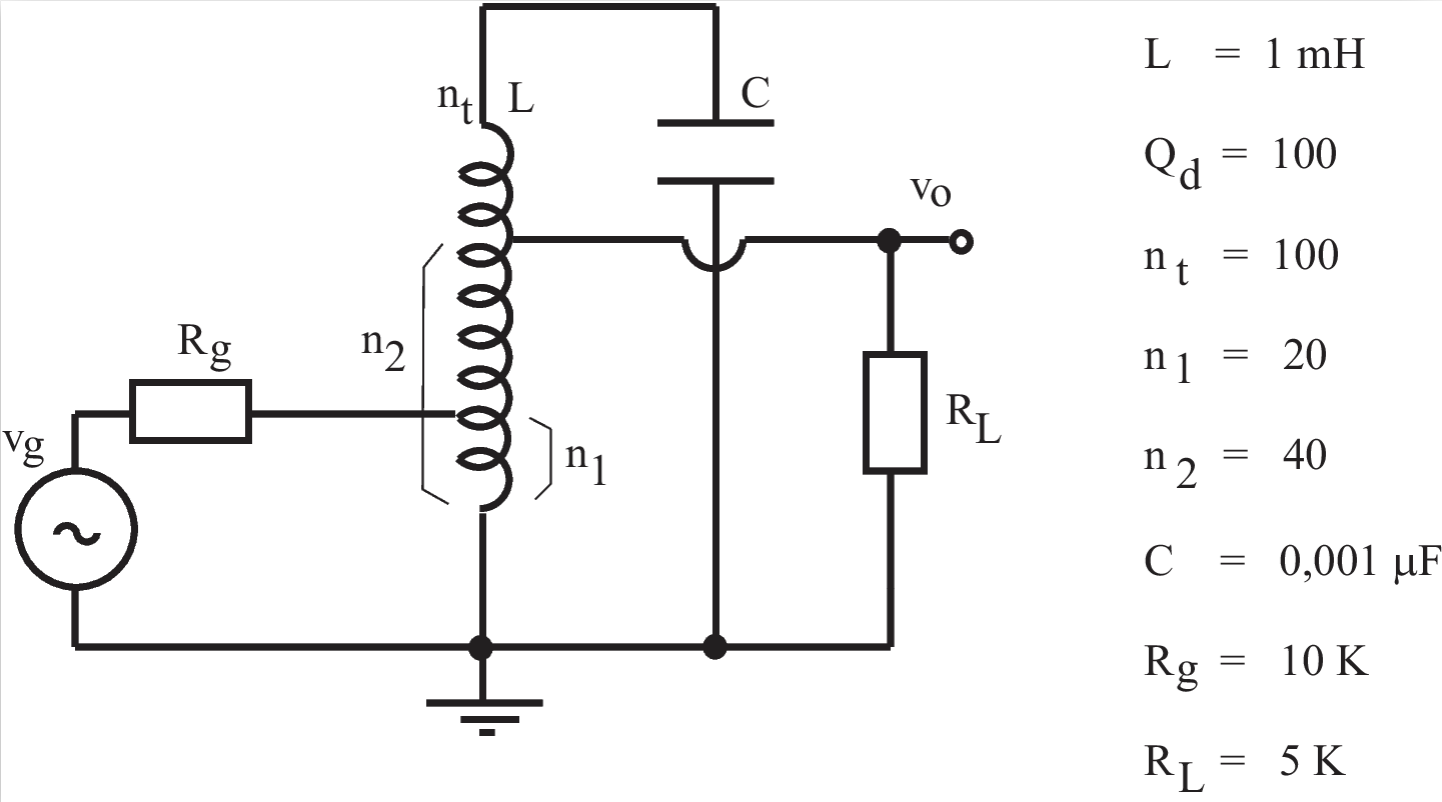
\includegraphics[width=0.6\linewidth]{figuras/sinto1.png}\\
	\caption{Ejercicio 1.}\label{sinto1}
\end{figure}


\textbf{Ejercicio 2}: El circuito de la figura \ref{sinto2} es un
amplificador de dos etapas de sintonía simple. Hallar la frecuencia
central, el ancho de banda total y la capacidad $C_1$. Hallar
también la expresión de la ganancia de tensión en función de la
frecuencia.

\begin{figure}[h]
	\centering
	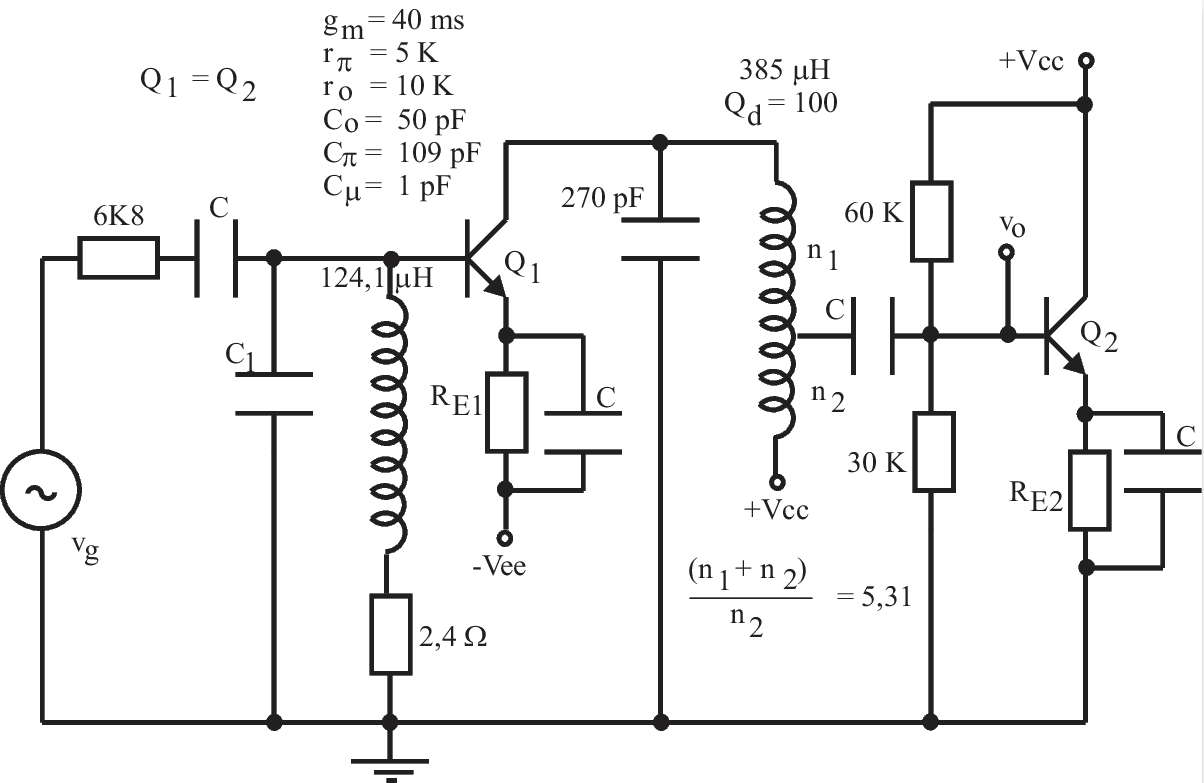
\includegraphics[width=0.8\linewidth]{figuras/sinto2.png}\\
	\caption{Ejercicio 2.}\label{sinto2}
\end{figure}



\textbf{Ejercicio 3}: Hallar la ganancia de tensión en función de la
frecuencia en el circuito equivalente de pequeña señal de la figura
\ref{sinto3}, denominado cascodo. Considerar además, que  ambas
etapas están sintonizadas a la misma frecuencia (calcular $C_x$ para
lograrlo). Explicar la ventaja de esta configuración con respecto
una en emisor común, y explicar por qué se utilizan transformadores
en lugar de bobinas.


\begin{figure}[h]
	\centering
	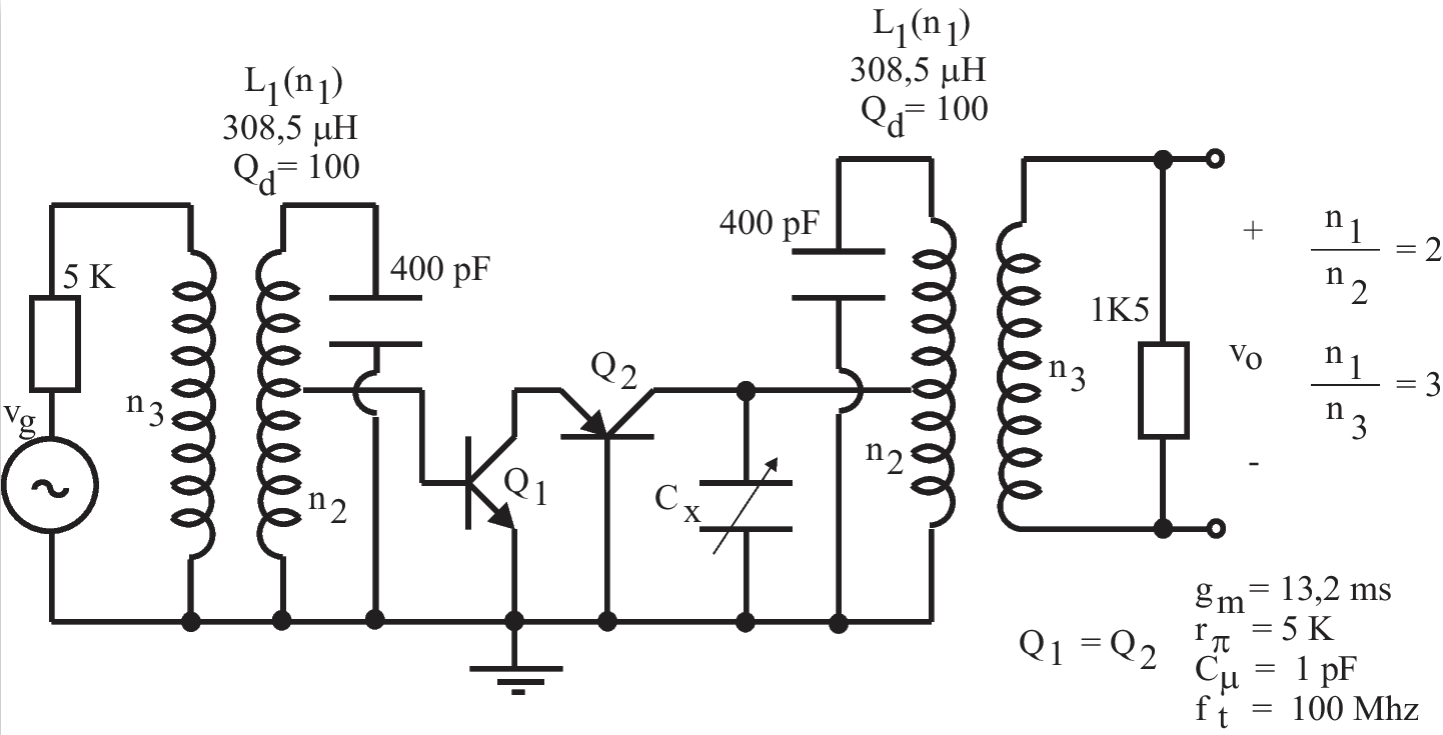
\includegraphics[width=0.8\linewidth]{figuras/sinto3.png}\\
	\caption{Ejercicio 3.}\label{sinto3}
\end{figure}



\textbf{Ejercicio 4}:  Hallar la ganancia de tensión y el ancho de
banda total del  circuito amplificador de la figura \ref{sinto4}. La
frecuencia de resonancia de cada etapa sintonizada se ajusta a 455
KH. Obtener los parámetros de los dispositivos a partir de las
condiciones de polarización.





\begin{figure}[h]
	\centering
	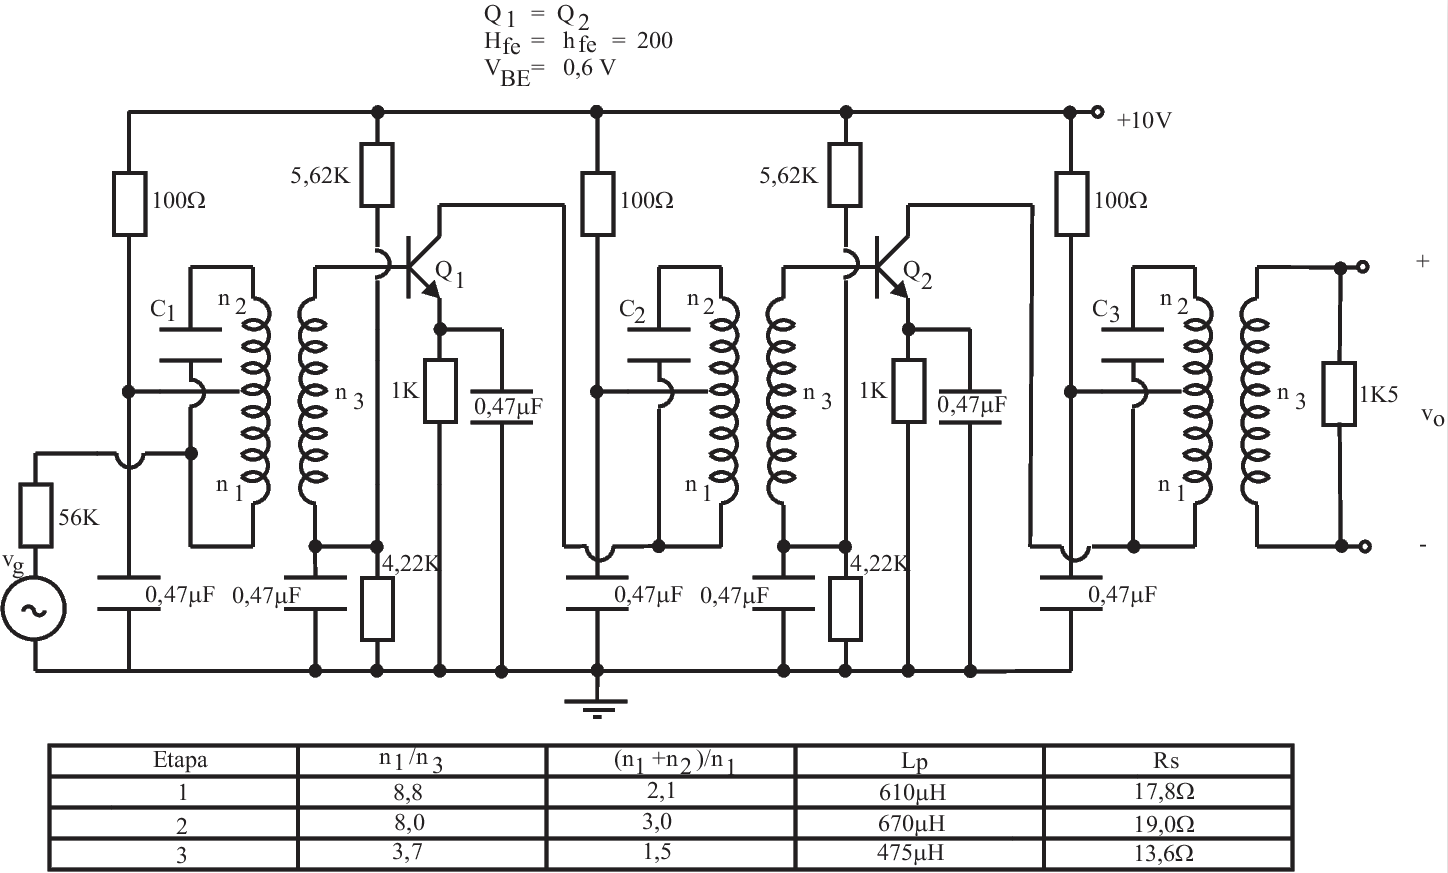
\includegraphics[width=0.9\linewidth]{figuras/sinto4.png}\\
	\caption{Ejercicio 4.}\label{sinto4}
\end{figure}

